\documentclass[11pt,a4paper]{article}
\usepackage[slovak]{babel}
\usepackage[utf8]{inputenc}
\usepackage[T1]{fontenc}
\usepackage{graphicx}
\usepackage{amsmath}
\usepackage{amssymb}
\usepackage{lmodern}
\usepackage{indentfirst}
\usepackage{titling}

\renewcommand{\labelenumi}{{\normalfont (\alph{enumi})}}
\renewcommand{\labelenumii}{{\normalfont \roman{enumii}.}}
\newcommand{\nN}{\ensuremath{\mathbb N}}
\newcommand{\nA}{\ensuremath{\mathcal A}}
%%%%%%%%%%%%%%%%%%%%%%%%%%%%%%%%%%%%%%%%%%%%%%%%%%%%%%%%%%%%%%%%%%%%%%%%%%%%%%%%
%%%                                                                          %%%
%%%%%%%%%%%%%%%%%%%%%%%%%%%%%%%%%%%%%%%%%%%%%%%%%%%%%%%%%%%%%%%%%%%%%%%%%%%%%%%%
\begin{document}
    %%%%%%%%%%%%%%%%%%%%%%%%%%%%%%%%%%%%%%%%%%%%%%%%%%%%%%%%%%%%%%%%%%%%%%%%%%%%%%%%
    %%%                                                                          %%%
    %%%%%%%%%%%%%%%%%%%%%%%%%%%%%%%%%%%%%%%%%%%%%%%%%%%%%%%%%%%%%%%%%%%%%%%%%%%%%%%%
    \title{Databázy (2) - Dátový model (1)}
    \author{Matej Kormuth, 2. ročník}
    %\date{}
    \date{\today}

    \begin{titlingpage}
        \renewcommand\maketitlehooka{\null\mbox{}\vfill}
        \renewcommand\maketitlehookd{\vfill\null}
        \maketitle
    \end{titlingpage}

    %%%%%%%%%%%%%%%%%%%%%%%%%%%%%%%%%%%%%%%%%%%%%%%%%%%%%%%%%%%%%%%%%%%%%%%%%%%%%%%%
    %%%                                                                          %%%
    %%%%%%%%%%%%%%%%%%%%%%%%%%%%%%%%%%%%%%%%%%%%%%%%%%%%%%%%%%%%%%%%%%%%%%%%%%%%%%%%
    \section*{ER model}

    Nalsedujúci diagram dokumentuje plánované entity a vzťahy medzi nimi.

    \begin{center}
        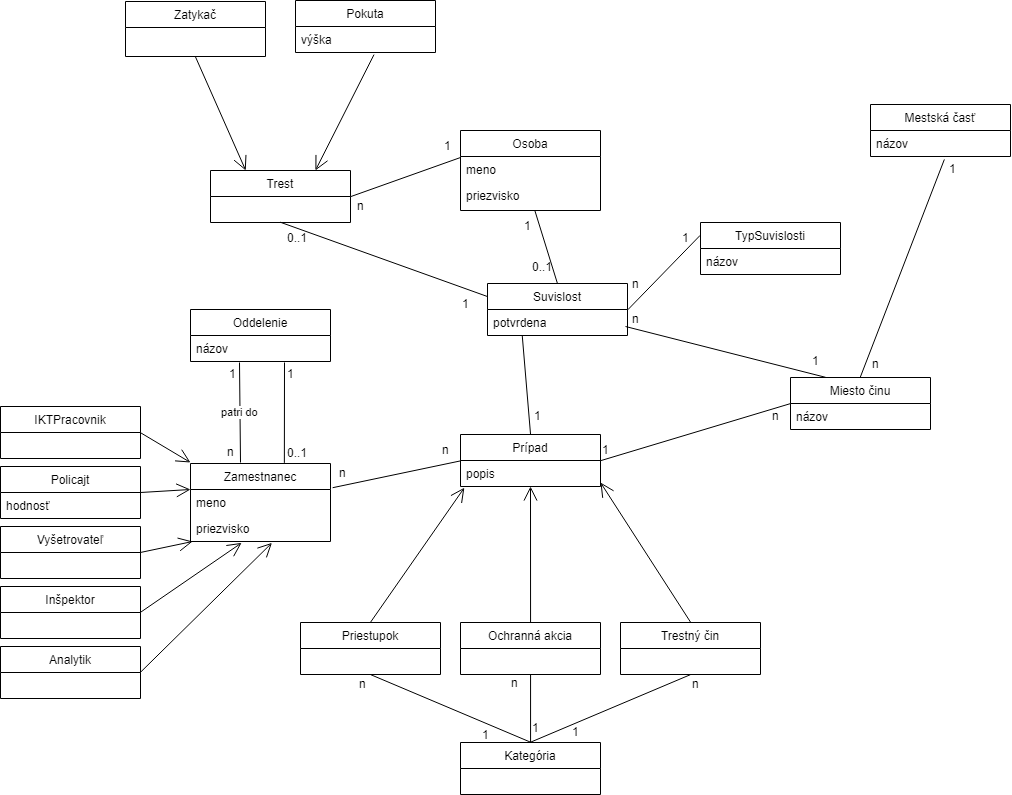
\includegraphics[width=\textwidth]{./model1.png}
    \end{center}

    Triedy IKTPracovník, Policajt, Vyšetrovateľ, Inšpektor a Analytik sú všetky potomkami Zamestnanca. Ak je zamestnanec Policajt, má aj svoju hodnosť.
    \\
    \\
    Každý zamestnanec je priradený do nejakého oddelenia a každé oddelenie má jedného vedúceho.
    \\
    \\
    Každý zamestnanec môže pracovať na veľa prípadoch, na jednom prípade môže pracovať viacero zamestnancov.
    \\
    \\
    Každý prípad je buď priestupok, trestný čin alebo orchranná akcia. Každý z nich má aj nejakú kategóriu. Každá kategória má svoje meno.
    \\
    \\
    V rámci jedného prípadu existuje veľa súvislostí. Jedna súvislosť súvisí práve s jednou osobou, jedným typom súvislosti (podozrivý, poškodený alebo svedok), jedným miestom činu a prípade že je potvrdená a je to súvislosť typu podozrivý aj s jedným trestom.
    \\
    \\
    Každé miesto činu patrí nejakej mestnej časti. Každé miesto činu má svoj názor / adresu. Každá mestská čast má svoj názov.
    \\
    \\
    Každá osoba môže dostať viacero trestov (z rôznych prípadov) a môže mať viacero súvislostí.
    \\
    \\
    Každý trest je buď zatykač alebo pokuta. Ak je to pokuta, tak má výšku. Každý trest súvisí s osobou, ktorej bol udelený vrámci nejakej súvislosti.
    \\
    \\
    %%%%%%%%%%%%%%%%%%%%%%%%%%%%%%%%%%%%%%%%%%%%%%%%%%%%%%%%%%%%%%%%%%%%%%%%%%%%%%%%
    %%%                                                                          %%%
    %%%%%%%%%%%%%%%%%%%%%%%%%%%%%%%%%%%%%%%%%%%%%%%%%%%%%%%%%%%%%%%%%%%%%%%%%%%%%%%%
\end{document}
%%%%%%%%%%%%%%%%%%%%%%%%%%%%%%%%%%%%%%%%%%%%%%%%%%%%%%%%%%%%%%%%%%%%%%%%%%%%%%%%
%%%                                                                          %%%
%%%%%%%%%%%%%%%%%%%%%%%%%%%%%%%%%%%%%%%%%%%%%%%%%%%%%%%%%%%%%%%%%%%%%%%%%%%%%%%%